\documentclass{sig-alternate}
\usepackage{epsfig}
\usepackage{algorithm}
\usepackage{algorithmic}

\title{Partitioning a Structured Stream Graph \\ Using Dynamic Programming}
\numberofauthors{1}
\author{
\alignauthor \vspace{-18pt}
William Thies,
Jasper Lin, and
Saman Amarasinghe \\
	\vspace{8pt}
	\{thies, jasperln, saman\}@lcs.mit.edu \\
	\vspace{8pt}
	Laboratory for Computer Science \\
	Massachusetts Institute of Technology}

\begin{document}

  \newtheorem{definition}{Definition}
  \newtheorem{transformation}{Transformation}
  
  \maketitle
  
  \newcommand{\mt}[1]{\mbox{\it #1}}
  \newcommand{\todo}[1]{\framebox{\bf #1}}
  
  \begin{abstract}
    As DSP programming is becoming more complex, there is an increasing
need for high-level abstractions that can be efficiently compiled.
Toward this end, we present a set of aggressive optimizations that
target linear sections of a stream program.  Our input language is
StreamIt, which represents programs as a hierarchical graph of
autonomous filters.  A filter is linear if each of its outputs can be
represented as an affine combination of its inputs.  Linear filters
are common in DSP applications; examples include FIR filters,
expanders, compressors, FFTs and DCTs.

We present a linear extraction analysis that automatically detects
linear filters based on the C-like code in their {\tt work} function.
Once linear filters are identified, we show how neighboring nodes can
be collapsed into a single linear representation, thereby eliminating
many redundant computations.  Also, we describe a method for
automatically translating linear nodes into the frequency domain,
thereby yielding algorithmic savings for convolutional filters.

We have completed a fully-automatic implementation of the above
techniques as part of the StreamIt compiler, and we demonstrate
performance improvements that average 400\% over our benchmark
applications.




  \end{abstract}

  \section{Introduction}

Applications that are structured around some notion of a ``stream''
are becoming increasingly important and widespread.  There is evidence
that streaming media applications are already consuming most of the
cycles on consumer machines \cite{Rix98}, and their use is continuing
to grow.  In the embedded domain, applications for hand-held
computers, cell phones, and DSP's are centered around a stream of
voice or video data.  The stream abstraction is also fundamental to
high-performance applications such as intelligent software routers,
cell phone base stations, and HDTV editing consoles.

Despite the prevalence of these applications, there is surprisingly
little language and compiler support for practical, large-scale stream
programming.  Of course, the notion of a stream as a programming
abstraction has been around for decades \cite{SICP}, and a number of
special-purpose stream languages have been designed (see
\cite{survey97} for a review).  Many of these languages and
representations are elegant and theoretically sound, but they often
lack features and are too inflexible to support straightforward
development of modern stream applications, or their implementations
are too inefficient to use in practice.  Consequently, most
programmers turn to general-purpose languages such as C or C++ to
implement stream programs.

There are two reasons that general-purpose languages are inadequate for
stream programming.  Firstly, they are a mismatch for the application
domain.  That is, they do not provide a natural or intuitive
representation of streams, thereby having a negative effect on
readability, robustness, and programmer productivity.  Moreover, because
the widespread parallelism and regular communication patterns of data
streams are left implicit in general-purpose languages, compilers are
not stream-conscious and do not perform stream-specific optimizations.
As a result, performance-critical loops are often hand-coded in a
low-level assembly language and must be re-implemented for each target
architecture.  This practice is labor-intensive, error-prone, and very
costly.

Secondly, general-purpose languages are a mismatch for the emerging
class of grid-based architectures \cite{smartmemories,rawshort,trips} that
are especially well-suited for stream processing.  Perhaps the primary
appeal of C is that it provides a ``common machine language'' for
von-Neumann architectures.  That is, it abstracts away the
idiosyncratic differences between machines, but encapsulates their
common properties: a single program counter, arithmetic operations,
and a monolithic memory.  However, for grid-based architectures, the
von-Neumann model no longer holds, as there are multiple instruction
streams and distributed memory banks.  Thus, C no longer serves as a
common machine language--in fact, it provides the wrong abstraction
for the underlying hardware, and architecture-specific directives are
often needed to obtain reasonable performance.  Again, this greatly
complicates the job of the programmer and hampers portability.

StreamIt is a language and compiler specifically designed for modern
stream programming.  The StreamIt language has two goals: first, to
provide high-level stream abstractions that improve programmer
productivity and program robustness within the streaming domain, and
second, to serve as a common machine language for grid-based
processors.  At the same time, the StreamIt compiler aims to perform
stream-specific optimizations to achieve the performance of an expert
programmer.

This paper motivates, describes, and justifies the high-level language
features of StreamIt, version 1.0.  The major limitation of StreamIt
1.0 is that all flow rates in the streams must be static; applications
such as compression that have dynamically varying flow rates will be
the subject of future work.  A large set of applications can be
implemented with static rates, and while dynamic rates will require a
different runtime model, it will still be essential to fully analyse
and optimize static sub-sections in order to obtain high performance.

The paper is organized as follows. In Section {\ref{sec:domain}}, we
characterize the domain of streaming programs that motivates the
design of StreamIt, and in Section~\ref{sec:overview} we describe the
language features in detail.  We present an in-depth example of a
software radio in Section~\ref{sec:example}, preliminary results in
Section~\ref{sec:results}, related work in Section~\ref{sec:related},
and conclusions in Section~\ref{sec:conc}.


  \section{StreamIt}
\label{sec:streamit}

StreamIt  is   an  architecture independent language that is
designed for  stream programming. In StreamIt, programs are
represented as graphs where  nodes represent  computation and edges
represent FIFO-ordered communication of data over tapes.

\paragraph*{Hierarchical Streams}
In  StreamIt, the  basic programmable  unit (i.e., an actor) is a {\it
filter}.   Each filter contains  a work  function that executes
atomically,  popping (i.e., reading)  a fixed number  of items  from
the  filter's input  tape and pushing (i.e., writing) a fixed number
of items to the filter's output tape.  A filter  may also {\tt peek} at
a given index  on its input tape without  consuming  the  item;  this
makes  it  simple  to  represent computation over a
sliding window.   The {\tt push}, {\tt pop}, and {\tt peek} rates are
declared as part  of  the work  function,  thereby enabling  the
compiler    to construct a static schedule of filter executions. The
following is an example implementation of a Finite Impulse
Response (FIR)  filter: 

\begin{scriptsize}
% {\small
\begin{verbatim}
float->float filter FIR (int N, float[] weights) 
{
  work push 1 pop 1 peek N {
    float sum = 0;
    for (int i = 0; i < N; i++) {
      sum += peek(i) * weights[i];
    }
    pop();
    push(sum);
  }
}
\end{verbatim}
% }
\end{scriptsize}

The work function is invoked (fired) whenever there is sufficient data
on the input tape. For the FIR example above, the filter requires at least
\texttt{N} elements before it can execute. The value of \texttt{N} is
known at compile time when the filter is composed to form a stream
graph. A filter is akin to a class in object oriented programming
with the work function serving as the main method. The parameters
to a filter (e.g., \texttt{N} and \texttt{weights}) are equivalent to
parameters passed to a class constructor. 

\begin{figure}[t]
\begin{center}
%\vspace{-24pt}
% \framebox{
 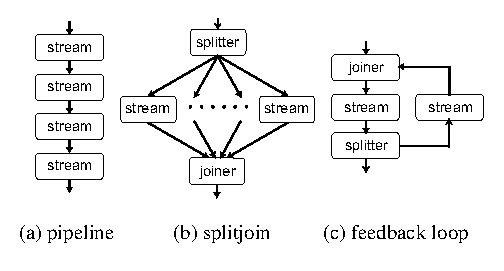
\includegraphics[scale=1, angle=0]{./constructs-eg.eps}
%}
% \vspace{-6pt}
% \nocaptionrule
 \caption{Hierarchical streams in StreamIt.}
 \label{fig:containers}
\end{center}
\end{figure}

\begin{figure}[t]
\begin{center}
\vspace{-12pt}
% \framebox{
 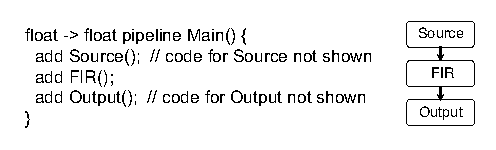
\includegraphics[scale=1, angle=0]{./pipeline-eg.eps}
%}
% \vspace{-6pt}
% \nocaptionrule
 \caption{Example pipeline with FIR filter.}
 \label{fig:pipeline}
%\vspace{-18pt}
\end{center}
\end{figure}

In StreamIt, the
application developer focuses on the hierarchical assembly of the
stream graph and its communication topology, rather than on the 
explicit management of the data buffers between filters.
StreamIt provides three hierarchical structures for composing filters
into larger stream graphs (see Figure~\ref{fig:containers}). The 
{\it pipeline} construct composes streams in sequence, with the output
of one connected to the input of the next.   An example of a pipeline
appears in Figure~\ref{fig:pipeline}.

The {\it splitjoin} construct distributes data to a set of parallel
streams, which are then joined together in a round robin fashion.  In
a splitjoin, the {\it splitter} performs the data scattering, and the
{\it joiner} performs the gathering. A splitter is a specialized
filter with a single input and  multiple output channels. On 
every execution step, it can distribute its output to any one of
its children in either a {\it duplicate} or a {\it roundrobin}
manner. For the former, incoming data are replicated to every
sibling connected to the splitter. For the latter, data are scattered
in a round robin manner, with each item sent to exactly one child
stream, in order.  The splitter type and the weights for distributing data to
child streams are declared as part of the syntax (e.g., \texttt{split
duplicate} or \texttt{split roundrobin($w_1,\ldots,w_n$)}). The
splitter counterpart is the joiner. It is a specialized filter with  
multiple input channels but only one output channel. The joiner
gathers data from its predecessors in a round robin manner (declared
as part of the syntax) to produce a single output stream.

StreamIt also provides a {\it feedback loop} construct for introducing
cycles in the graph.

%\section{Execution Model}
%\label{sec:execmodel}

%% A StreamIt program is represented by a hierarchical graph,
%% where the leaf nodes are filters, splitters, and joiners, and
%% the composite nodes are pipelines, splitjoins, and
%% feedback-loops. Edges in the graph represent data channels, which 
%% operate as FIFO queues.
\paragraph*{Execution Model}
As noted earlier, an actor (i.e., a filter, splitter, or joiner)
executes whenever there are enough data items on its input 
tape. In StreamIt, actors have  two epochs
of execution: one for initialization, and one for the {\it steady
state}. The initialization primes the input tapes to allow filters with
peeking to execute the very first instance of their work functions.
%%initialization in this setting is similar to the prologue stage in
%%software pipelining. 
A steady state is an execution that does not change the
buffering in the channels: the number of items on each channel
after the execution is the same as it was before the execution. 
Every valid stream graph has a steady state~\cite{LM87-i}, and within
a steady state, there are often many possibilities for interleaving
actor executions. 
%% The steady state schedule has the property that
%% the amount of data buffered between any two actors does not change
%% before and after the actor executions.
\begin{figure}[t]
\begin{center}
%%\vspace{-24pt}
%\vspace{24pt}
 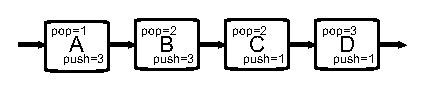
\includegraphics[scale=1, angle=0]{./pipe-with-rates.eps}
%\vspace{-6pt}
% \nocaptionrule
 \caption{Example pipeline.}
 \label{fig:pipe-with-rates}
\end{center}
%\vspace{-12pt}
\end{figure}
An example of a steady state for the pipeline in
Figure~\ref{fig:pipe-with-rates} requires filter \texttt{A} to fire
4 times, \texttt{B} 6 times, \texttt{C} 9 times, and
\texttt{D} 3 times. 
% Because in StreamIt the filters are
% independent (i.e., they do not share state), they can execute
% concurently. In a uniprocessor setting (which is what we use for our
% evaluation), we can only run one filter at time. Therefore, 
% The data generated by one actor are buffered (cached) until they are
% consumed.

\paragraph*{Compilation Process}
The StreamIt compiler derives the initialization and steady state
schedules~\cite{karczma-lctes03} and outputs a C program that includes
the initialization and work functions, as well as a driver to execute
each of the two schedules. Our compilation process allows the StreamIt
compiler to focus on high level optimizations, and relies on existing
compilers to perform machine-specific optimizations such as register
allocation, instruction scheduling, and 
code generation---this two step approach affords us a
great deal of portability (e.g., code generated from the StreamIt
compiler is compiled and run on three different machines as reported
in Section~\ref{sec:evaluation}).

%% For example, referring to
%% Figure~\ref{fig:pipe-with-rates}, the compiler generates the following
%% sample code for running the steady state schedule:
%% %\begin{scriptsize}
%% \begin{verbatim}
%% run_steady_state() {
%%   for (i = 0; i < 4; i++) A_work();
%%   for (i = 0; i < 6; i++) B_work();
%%   for (i = 0; i < 9; i++) C_work();
%%   for (i = 0; i < 3; i++) D_work();
%% }
%% \end{verbatim}
%% %\end{scriptsize}
%% To execute the program, the steady state is wrapped with
%% another loop that invokes the steady state a designated number of
%% times. Preceding the state steady, a similar initialization schedule
%% is run to prime the data buffers.
%, and following the steady state, an
%epilogue is run to drain the buffers as necessary.

%% \begin{figure}[t]
%% \begin{center}
%% \vspace{-12pt}
%%  \psfig{figure=ssi.eps,width=3in}
%%  \vspace{-6pt}
%%  \caption{Instruction size (in bytes along the y-axis) per filter
%%  (x-axis) occurring in a steady state execution of FFT.}
%%  \label{fig:ssi-single}
%% \vspace{-18pt}
%% \end{center}
%% \end{figure}

  
\section{Graph Transformations}

In this section we present a set of flexible transformations that can
be used to adjust the hierarchy and communication patterns of a
structured stream graph.  These transformations serve two purposes.
Firstly, they provide a means of deriving a canonical form: a program
representation that is insensitive to changes in the source code and
is easily analyzed by the compiler.  Secondly, they serve as the
implementation mechanism by which the compiler arrives at an efficient
executable once it has analyzed the canonical form.  Thus, we consider
the transformations in pairs, each of which represents respresents a
step in the opposite direction with respect to the canonical form.

\subsection{Vertical Cut Transformations}

The vertical cut transforms effect the distribution of parallel
streams across a hierarchy of splitjoin constructs (see
Figures~\ref{code:vert} and~\ref{ex:vert}).  The {\tt lowerChildren}
transform can factor any adjacent subset of a splitjoin's children
into a new splitjoin, which becomes a child of the original.  This is
a simple matter of re-arranging the weights in the splitters and
joiners.  It qualifies as a ``vertical cut'' transform because two
adjacent applications can divide a splitjoin with a vertical line.

The {\tt raiseChildren} transform will reverse the effect of any {\tt
lowerChildren} transform.  However, independent applications of this
transform are comparably rare: as detailed in the pseudocode, a child
can only be raised if its splitter type matches that of its parent,
and if the sums of its split and join weights match the corresponding
slots in the parent.

\subsection{Horizontal Cut Transformations}

The horizontal cut transforms are capable of transforming between a
splitjoin and a pipeline of splitjoins (see Figures~\ref{code:horiz}
and~\ref{ex:horiz}).  The {\tt addMatchingSyncPoints} transformation
inputs a rectangular splitjoin--one with pipeline children that have
equal lengths--and factors them into a sequence of splitjoins with
children that have unit length.  For the purpose of program analysis,
any splitjoin can be made rectangular by extending its shorter streams
with {\tt Identity} filters (a pre-defined node in StreamIt.)  Like an
hourglass, this transformation has the effect of squeezing a splitjoin
together at points of synchronization.

The {\tt removeMatchingSyncPoints} transformations directly implements
the inverse of {\tt addMatchingSyncPoints} via a simple re-arrangment
of weights.  Though very simple, this transformation can apply in
practice on interface boundaries where compound data streams are being
interleaved at a static rate.

A more aggressive transformation for synchronization removal is {\tt
removeStructuredSyncPoints} (see Figures~\ref{code:sync1}
and~\ref{code:sync2}).  This algorithm removes not only
synchronization points with exactly matching weights, but it also
expands any join/split pair where the set of incoming and outgoing
streams can be partitioned such that no data item is passed between
members of different partitions during a steady-state execution.  The
only disadvantage of this transformation over {\tt
removeMatchingSyncPoints} is that it has the potential to introduce
non-adjacent joiners, which in the StreamIt compiler requiers
additional processor resources.  However, like all transformations
described in this paper, the output of {\tt
removeStructuredSyncPoints} is still a structured graph (as the name
would suggest).

\subsection{Fusion and Fission Transformations}

Filter fusion describes a transform where several adjacent filters are
combined into one, while filter fission refers to the parallelization
of a filter via conversion to a splitjoin or pipeline.  These
transformations are at the heart of the load balancing partitioner
described in this paper.  A detailed description of fusion, fission,
and other intra-node transformations are described
in~\cite{streamit-asplos}; we restrict our attention to graph-level
transformations in this paper.

%  what is the algorithm with time partitioning?

I guess, just add the bottleneck work from each of the time
partitions?

have to guarantee that time partitions are on the outside...

-----------------

\section{Partitioning}

\scriptsize
\begin{verbatim}

structures
----------
container s:
  s.width()    : returns width of rectangle
  s.length()   : returns length of rectangle
  s.get(i, j)  : returns the (i,j)'th child


globals
-------
// A_s[x1][x2][y1][y2][n] holds minimum cost of assigning children 
// (x1..x2, y1..y2) of stream s to n tiles
forall s in graph:  int[][][] A_s;


// setup for n partitions
void setup(int n) 
-----------------
(lift all redundant pipelines / splitjoins)
(consider feedbackloops as a 2-way splitjoin, each child of which is a
 1-way splitjoin to prevent introducing synchronization across the loop
 and body segments.)
(eliminate all pipelines in splitjoins in favor of rectangular splitjoins)
(pad all splitjoins so that each parallel stream is same length)

forall s in graph
  A_s = new int[s.length()][s.length()][s.width()][s.width()][n]
  forall (x1,x2,y1,y2,n) \in A_s
    A[x1][x2][y1][y2][n] = -1


// returns whether or not stream <s> needs a joiner if it is spread
// across multiple tiles
boolean needsJoiner (stream s)
------------------------------
par = s.parent()
if (par==null)
  // if have no parent, then need a joiner
  return true
else if (par.width()>1)
  // if par has multiple streams, it will have joiner instead
  return false;
else if (par.parent()==null && s!=par.get(0, par.length()-1))
  // if we're in middle of toplevel stream, then need joiner
  return true
else
  // otherwise we're guaranteed by lifter that par.parent().width>1,
  // so there will be a joiner there and we don't need one for s
  return false
end if


// return minimal cost for allocating <n> partitions to children
int getCost(stream s, int n)
----------------------------

// see if we will need a joiner
if (n>1 && needsJoiner(s)) 
  n--
endif

if (s is Node)
 return getNodeCost(s, n)
if (s is Container)
 return getContCost(s, 0, s.width()-1, 0, s.length()-1, n)


int getContCost(stream s, int x1, int x2, int y1, int y2, int n)
----------------------------------------------------------------
// if value is memoized, return it
if (A_s[x1][x2][y1][y2][n] != -1)
  return A_s[x1][x2][y1][y2][n]
endif

// if down to one child, descend into it
if (x1==x2 && y1==y2)
  int cost = getCost(s.get(x1, y1), n)
  A_s [x1][x2][y1][y2][n] = cost
  return cost;
endif

// if n is 1, just sum the work of components
if (n==1)
  int sum = getContCost(s, x1, x1, y1, y1, n);
  sum += x1<x2 ? getContCost(s, x1+1, x2, y1, y1, n) : 0
  sum += y1<y2 ? getContCost(s, x1, x1, y1+1, y2, n) : 0
  sum += x1<x2 && y1<y2 ? getContCost(s, x1+1, x2, y1+1, y2, n) : 0
  return sum
endif

// try making vertical cut (in case s is a splitjoin)
int min = infinity
for xPivot = x1 to x2 - 1
  for nPivot = 1 to n-1
    int cost = max(getContCost(s, x1, xPivot, y1, y2, nPivot),
                   getContCost(s, xPivot+1, x2, y1, y2, n-nPivot));
    if (cost < min)
      min = cost
    endif
  endfor
endfor

// try making horizontal cut (for splitjoin, pipeline, feedbackloop)
for yPivot = y1 to y2 - 1
  for nPivot = 1 to n-1
    int cost = max(getContCost(s, x1, x2, y1, yPivot, nPivot),
                   getContCost(s, x1, x2, yPivot+1, y2, n-nPivot));
    if (cost < min)
      min = cost
    endif
  endfor
endfor

A[x1][x2][y1][y2][n] = min;
return min


// returns cost of node <s> assigned to <n> tiles
int getNodeCost(stream s, int n)
--------------------------------
if (isFissable(s))
  return work / n
else
  return work
endif


// traceback and construct a mapping <map> from nodes to partitions.
// <assigned> represents the number of partitions assigned so far.
void traceback(stream s, list-of (stream,int) map, int assigned, int n)
---------------------------------------------------------------
if (s is Node)
  tracebackNode(s, map, assigned, n)
if (s is Container)
  tracebackCont(s, map, assigned, 0, s.width()-1, 0, s.length()-1, n)


// traceback for node
void tracebackNode(stream s, list-of (stream,int) map, int assigned, int n)
---------------------------------------------------------------
for i = 0 to n-1
  map.append(s, assigned+i)
endfor


// traceback for container
void tracebackCont(stream s, list-of (stream,int) map, int assigned, 
                   int x1, int x2, int y1, int y2, int n)
---------------------------------------------------------------
// if we only have one partition left, or if we are only
// looking at one child, then just recurse into children
if (tileLimit==1 || (x1==x2 && y1==y2))
  for i = x1 to x2
    for j = y1 to y2
      traceback(s.get(i,j), map, assigned, n);

// otherwise, see if we made a vertical cut (in case s is a splitjoin)
int min = infinity
for xPivot = x1 to x2-1
  for nPivot = 1 to n-1
    int cost = max(getContCost(s, x1, xPivot, y1, y2, nPivot),
                   getContCost(s, xPivot+1, x2, y1, y2, n-nPivot));
    if (cost==A[x1][x2][y1][y2][n]) {
      // found best cost, so there's a division at this <xPivot>.  Recurse
      // left and right, incrementing assignment count after partition.
      traceback(s, map, assigned, x1, xPivot, y1, y2, nPivot)
      traceback(s, map, assigned+nPivot, xPivot+1, x2, y1, y2, n-nPivot);
      return
    endif
  endfor
endfor

// try making horizontal cut (for splitjoin, pipeline, feedbackloop)
for yPivot = y1 to y2 - 1
  for nPivot = 1 to n-1
    int cost = max(getContCost(s, x1, x2, y1, yPivot, nPivot),
                   getContCost(s, x1, x2, yPivot+1, y2, n-nPivot));
    if (cost==A[x1][x2][y1][y2][n]) {
      // found best cost, so there's a division at this <yPivot>.  Recurse
      // left and right, incrementing assignment count after partition.
      traceback(s, map, assigned, x1, x2, y1, yPivot, nPivot)
      traceback(s, map, assigned+nPivot, x1, x2, yPivot+1, y2, n-nPivot);
      return
    endif
  endfor
endfor


// do partitioning of stream s on n tiles and return mapping from node
// to partition number
stream->int toplevel(stream s, int n)
-------------------------------------
setup(n)
cost = getCost(s, n)

// if desired, eliminate extra partitions that aren't contributing to
// the cost
while (n>1 && getCost(s, n-1)==cost)
  n--
endwhile

traceback(s, empty-map, 0, n)

return map

\end{verbatim}

  \section{Experimental Evaluation}

In this section we present an evaluation of the contributions of this
paper and compare to previous techniques for compiling stream programs
to multicore architectures.  This section will include an elaboration
of the following contributions and conclusions:

\begin{itemize}
\item Our technique for exploiting coarse-grained data parallelism
produces abundant parallelism and achieve a geometric mean performance
gain of 9.9x over a strictly task parallel baseline.
\item Coarse-grained software pipelining is a
an effective technique for extracting parallelism beyond task and data
parallelism, with an additional geometric mean speedup of 1.45x. On
its own, our software pipelining technique affords a 7.7x performance
gain over a task parallel baseline.
\item The combination of the techniques presented in this paper
improves upon previous work that exploited a combination of task and
pipeline parallelism.
\end{itemize}

First, we present a description of the benchmark suite employed
in the evaluation.

\begin{figure*}[t]
\centering
\psfig{figure=benchchar.eps, width=6.5in}
\caption{Benchmark characteristics
\protect\label{fig:benchchar}}
\end{figure*}

\subsection{Benchmark Suite}
We evaluate our techniques using the benchmark suite given in Figure
\ref{fig:benchchar}.   The benchmark suite consists of 12 StreamIt
applications. MPEG2Decoder implements the block decoding and the
motion vector decoding of an MPEG-2 decoder, containing approximately
one-third of the computation of the entire MPEG-2 decoder.  Also, the
DCT benchmark implements a 16x16 IEEE reference DCT while the
MPEG2Decoder benchmark includes an 8x8 IEEE fast DCT as a component.
For additional information for MPEG2Decoder, Vocoder, and Radar,
please refer to \cite{ipdps2006},
\cite{seneff80}, and \cite{pca}, respectively. 

In the table, the measurements given in each column are obtained from
the stream graph graph as conceived by the programmer, before it is
transformed by our techniques.  The ``Filters'' columns gives the
total number of filters in the stream (including file input filters
and file output filters that are not mapped to cores).  The number of
filters that perform peeking is important because peeking filters
cannot be fused without introducing shared state.  Thus, once a
peeking filter is fused, it cannot be fissed. In the table, the column
labeled ``Shortest Path'' and ``Longest Path'' give the shortest path
and the longest, path from source to sink. ``Comp / Comm'' gives the
static estimate of the computation to communication ratio of each
benchmark for one steady-state execution. This is calculated by
totaling the computation estimates across all filters and dividing by
the number of items communicated per steady-state. Notice that
although the computation to communication ratio is high across our
benchmarks, we demonstrate that inter-core synchronization is an
important factor to consider.

The benchmarks are sorted in ascending order of the final column,
``Stateful work''. This is percentage of the statically estimated work
performed per steady-state by all filters that have state divided by
the total work performed by all filters per steady-state.  Referring
to Figure \ref{fig:benchchar}, we see that three of our benchmarks
include stateful computation.  The stateful computation performed in
MPEGDecoder is insignificant and expressed as...
\textbf{Bill, can you talk about the statefull computation in
MPEG, radar, and vocoder}.


\begin{figure*}[t]
\centering
\psfig{figure=maingraph.eps, width=6.5in}
\caption{Task, Task + Data, and Task + Data + Software Pipeline
\protect\label{fig:main_comp}}
\end{figure*}

\subsection{Exploiting Coarse-Grained Data Parallelism}
To motivate the necessity of our parallelism extraction techniques let
us first consider the task parallel execution model.  This model
closely approximates a thread model of execution where the only form
of coarse-grained parallelism exploited is fork/join parallelism.  In
our implementation, the sole form of parallelism exploited in this
technique is the parallelism across the children of a splitjoin. The
first bar of Figure \ref{fig:main_comp} gives the throughput speedup
of the each of our benchmarks running in the task parallel model
executing on 16-core Raw normalized to sequential StreamIt executing
on a single core of Raw.  For the remainder of the presentation,
unless otherwise noted, we target all 16 cores of Raw.  The geometric
mean performance speedup for task parallel is 2.27x over sequential
performance. We can see that for most of our benchmarks, little
parallelism is exploited, notable exceptions are Radar,
ChannelVocoder, and FilterBank.  Each contains wide splitjoins of
load-balanced children.  In the case of BitonicSort, the task
parallelism is expressed at too fine a granularity for the
communication system.  Given that we are targetting a 16-core
processor, a mean speedup of 2.27x is inadequate.

The StreamIt programming model facilitates relatively simple analysis
to determine opportunities for data parallelism.  But the granularity
of the transformations must account for the additional synchronization
incurred by data-parallelizing a filter.  If we attempt to exploit
data-parallelism a fine granularity, by simply replicating each
stateless filter across the cores of the architecture we run the risk
of overwhelming the communication substrate of the target
architecture.  To study this, we implemented a simple algorithm for
data parallelism, replicate each filter by the number of cores,
mapping each to its own core.  In
\ref{fig:fine-dup}, we show this technique normalized to single-core
performance.  \textbf{todo!}

The second bar of Figure \ref{fig:main_comp} gives the speedup of
coarse-grained data parallelism over single-core StreamIt. The mean
speedup across our suite is 9.9x over single-core and 4.36x over our
task parallel baseline (not shown in the figure).  BitonicSort, whose
original granularity was too fine, now achieves a 8.4x speedup over a
single-core. 6 of our 12 applications are stateless and non-peeking,
and thus fuse to one filter that is fissed 16 ways.  For these
benchmarks the mean speedup is 11.1x over the single-core.  For DCT,
the algorithm data-parallelizes the bottleneck of the application (a
single filter that performs more than 6x the work of each of the other
filters).  For DCT, coarse-grained data parallelism achieves a 14.6x
speedup over single-core, while fine-grained achieves only 4.0x
because it fisses at too fine a granularity, improperly considering
synchronization.  Coarsening and then parallelizing reduces the
synchronization costs of data parallelizing.  For Radar and Vocoder,
data parallelism is paralyzed by the preponderance of stateful
computation.

\subsection{Exploiting Coarse-Grained Software Pipeline Parallelism}

\begin{figure}[t]
\centering
\psfig{figure=softpipe_graph.eps, width=3.2in}
\caption{Task and Task + Software Pipeline
\protect\label{fig:softpipe_graph}}
\end{figure}
Our novel technique for coarse-grained software pipelining is
effective for exploiting coarse-grained parallelization (though it
under-performs when compared to coarse-grained data parallelism).
More importantly, combining software pipelining with our data
parallelism techniques, provides a cumulative performance gain,
most especially for applications with stateful computation.

Figure \ref{softpipe_graph} considers coarse-grained software
pipelining and task parallelism normalized to single-core performance.
On average, software pipelining has a speedup of 7.7x over single-core
(compare to 9.9 for data parallelism) and a speedup of 3.4x over task
parallelism. Software pipelining performs well when it can effectively
load-balance the packing of the dependence-free steady-state.  In the
case, of Radar, TDE, FilterBank, and FFT, software pipelining achieves
comparable or better performance compared to data parallelism (see
Figure \ref{fig:thruput}).  For these applications, the workload is
not dominated by a single filter and the resultant schedules are
statically load-balanced across cores.  For the Radar application,
software pipelining achieves a 2.3x speedup over data parallelism and
task parallelism because there is little coarse-grained data
parallelism to exploit and it can more effectively schedule the
dependence-free steady-state.

However, when compared to data parallelism, software pipelining is
hampered by its inability to reduce the critical path when the
critical path contains stateless work (e.g., DCT, MPEGDecoder).  Also,
our data parallelism techniques tend to coarsen the stream graph more
than Selective Fusion, removing more synchronization.  For example, in
DES, the Selective Fusion Algorithm makes a greedy decision that it
cannot remove communication affecting the critical path workload.
Software pipelining performs poorly for this application when compared
to data parallelism, 6.9x versus 13.9x over single core, although it
calculates a load-balanced mapping.  Another consideration when
comparing software pipelining to data parallelism is that the software
pipelining techniques rely more heavily on the accuracy of the static
work estimation strategy, although it is difficult to quantify this
effect.

When we software pipeline the data-parallelized stream graph, we
achieve a 45\% mean speedup over data parallelism alone. The
cumulative effect is most prominent when the application in question
contains significant amounts of stateful computation.  For example,
the combined technique achieves a 69\% speedup over each individual
technique for Vocoder. For most of our other applications, software
pipeline further coarsens the stream graph without affecting the
critical path work (as estimated statically) and performs inter-core
communication in parallel.  Each reduces the synchronization
encountered on the critical path.

The combined technique depresses the performance of MPEG by 6\%
because the Selective Fusion component of the software pipeliner fuses
one step too far.  In most circumstances, fusion will help to reduce
inter-core synchronization by using the local memory of the core for
buffering. Consequently, the algorithm does not model the
communication costs of each fusion step. In the case of MPEG, it fuses
too far and adds synchronization by fusing two elements of a splitjoin
that perform little work.  The combined filter communicates more data
across the splitjoin than its sibling (who perform much more work).
The critical path of the application is increased because the
synchronization cost of splitting and joining increases.  The combined
technique also hurts Radar as compared to only software pipelining
because we fiss too aggressively and create synchronization across the
critical path.

In Figure \ref{fig:thruput}, we report the compute utilization and the
MFLOPS performance for each benchmark employing the combination of our
techniques. Note that for our target architecture, the maximum number
of MFLOPS achievable is 7200.  The compute utilization is calculated
as the number of instructions issued on each computer processor
divided by the total number possible for a steady-state.  The
utilization accurately models pipeline hazards and stalls of Raw's
single issue, in-order processing cores.  We achieve generally
excellent compute utilization; in 7 cases the utilization is 60\% or
greater.


\subsection{Comparison To Previous Work}

\begin{figure}[t]
\centering
\psfig{figure=vs_space_graph.eps, width=3.2in}
\caption{Task + Pipeline and Task + Data + Software Pipeline
\protect\label{fig:vs-space}}
\end{figure}

\begin{figure*}[t]
\centering
\psfig{figure=thruput.eps, width=6.5in}
\caption{Comparison and Task + Data + Software Pipeline Performance Results
\protect\label{fig:thruput}}
\end{figure*}
In Figure \rev{fig:vs-space} we show our combined technique normalized
to our previous work \cite{streamit-asplos}.  

Space good versus us for applications composed of long pipelines with little
splitting, including FFT5, tde

Serpent is fused down to a load-balanced pipeline, splitjoins
composed in a pipeline, space version has util of 64\% we are fusing
then taking advantage of pipeline parallelism, not always the right
thing to do.

Talk more about using on-chip network

Also the way we simulate input differs between the two backends.  Task
+ Pipeline attaches the input and output devices to the chip in the
place of dram, and the input is continuously streamed onto the chip.
The new backend fetches input and writes output from/to the DRAMs,
generating a DRAM command.

Raw's on-chip network is well-suited to pipeline communication, but it
does not approximate any other multicore.

DCT: must be partitioned to 16 tiles, the bottleneck is fissed 2 ways,
but the remaining stages must be fused to 4-way and they become the
bottleneck, plus synchronization!

MPEG: space partitioner must fuse down to 16 tiles removing task
parallelism of the program, and the work is not evenly distributed
across the application, resulting partitioning is not load-balanced,
dominated by a single filter that does more than 2x the amount of work
than the next largest filter.

DES:somewhat complicated graph repeated 4 time between some filters,
space partitioner is forced to partition these 4 containers (8 filters
each) into 2 filters that are not load balanced.  Synchronization
issues not alleviated when forced to fuse to pipeline.

Stateful benchmarks, compare without softpipe to space, and
then softpipe kicks in, hopefully, like 
vocoder:
beamformer:Task + Data loses to space by 19\%, T+D+SP beats space by
38\%
vocoder:T+D loses to space by 18\%, T+D+SP beats space by 30\%.


  \section{Non-Hierarchical  Transformations}

\section{Non-Hierarchical Graph Transformations}

\subsection{Vertical SplitJoin Fission}

Can pull out a node from a splitjoin.

\subsection{}

\subsection{Unstructured Syncronization Removal}


\section{Non-Hierarchical Cost Functions}

\subsubsection{Layout}

\subsubsection{Communication}






  \begin{figure}[t]
    \psfig{figure=algorithm4.eps,width=3.5in}
    \caption{Refactoring hierarchical splitjoin children.}
  \end{figure}
  
  \begin{figure}[t]
    \psfig{figure=algorithm5.eps,width=3.5in}
    \caption{Adding and removing splitjoin synchronization.}
  \end{figure}
  
  \begin{figure}[t]
    \psfig{figure=algorithm6.eps,width=3.5in}
    \caption{Aggressive synchronization removal.}
  \end{figure}
  
  \clearpage
  \begin{figure*}[t]
    \begin{tabular}{ll}
    \psfig{figure=algorithm.eps,width=3.5in}
    &
    \psfig{figure=algorithm2.eps,width=3.5in}
    \end{tabular}
    \caption{Search phase of the partitioning algorithm.  The traceback phase appears in the appendix.
      \protect\label{code:partition}}
  \end{figure*}

  \section*{Appendix}
  \clearpage
  \begin{figure}[t]
    \psfig{figure=algorithm3.eps,width=3.5in}
  \end{figure}
  
  % Bibliography -- whee!
  \begin{small}
    \bibliographystyle{abbrv}
    \bibliography{references}
  \end{small}
  
\end{document}